\documentclass[12pt,a4paper]{article}
\usepackage[utf8]{inputenc}
\usepackage[margin=1in]{geometry}
\usepackage{graphicx}
\usepackage{float}
\usepackage{amsmath}
\usepackage{listings}
\usepackage{xcolor}
\usepackage{enumitem}

% Code listing style
\lstset{
    language=C++,
    basicstyle=\ttfamily\footnotesize,
    keywordstyle=\color{blue},
    commentstyle=\color{green},
    stringstyle=\color{red},
    numbers=left,
    numberstyle=\tiny,
    frame=single,
    breaklines=true
}

\begin{document}

% Front Page
\begin{titlepage}
  \centering
  \vspace*{3cm}

  {\Huge\bfseries CSE 406 – Lab Report 5: Disk Scheduling using SSTF (Shortest Seek Time First) \par}
  \vspace{2.5cm}

  \noindent
  \begin{minipage}[t]{0.48\textwidth}
    {\large\bfseries Submitted By:}\\[0.5em]
    \Large
    Sharif Md. Yousuf \\
    ID: 22101128 \\
    Section: C-2 \\
    4th Year, 1st Semester \\
    Spring 2025
  \end{minipage}
  \hfill
  \begin{minipage}[t]{0.48\textwidth}
    {\large\bfseries Submitted To:}\\[0.5em]
    \Large
    Atia Rahman Orthi \\
    Lecturer \\
    Department of Computer Science \& Engineering \\
    University of Asia Pacific
  \end{minipage}

  \vfill

  {\Large\bfseries Date of Submission:} \\[0.5em]
  {\LARGE\bfseries 16 August, 2025 (Saturday)}

  \vspace*{2cm}
\end{titlepage}

\section{Problem Statement}
Implement a disk head scheduling simulator for the Shortest Seek Time First (SSTF) algorithm. Given an initial head position and a list of pending cylinder requests, at each step the algorithm must select the unfinished request with the minimum absolute seek distance from the current head location. The program outputs the order in which requests are served, the individual head movements, the total head movement, and the average seek per serviced request.

\subsection*{Input}
\begin{itemize}
  \item First line: two integers $n$ and $head$ where $n>0$ is the number of requests and $head$ is the initial cylinder position.
  \item Next either:
    \begin{itemize}
      \item A single line containing $n$ integers (space separated), or
      \item $n$ lines each containing one integer.
    \end{itemize}
  Each integer is a non-negative cylinder number.
\end{itemize}

Example inputs (both equivalent forms):
\begin{verbatim}
8 50
176 79 34 60 92 11 41 114
\end{verbatim}
or
\begin{verbatim}
8 50
176
79
34
60
92
11
41
114
\end{verbatim}

\subsection*{Output}
\begin{itemize}
  \item Line: Initial head position.
  \item Line: The order in which requests are serviced (SSTF sequence) separated by arrows.
  \item A table showing per-move index, from, to, and movement distance.
  \item Two summary lines: total head movement and average seek per move (formatted to two decimals).
\end{itemize}

Illustrative output fragment:
\begin{verbatim}
Initial Head: 50
Request Order (SSTF served):
41 -> 34 -> 60 -> 79 -> 92 -> 114 -> 176 -> 11

Index	From	To	Move
1	50	41	9
...

Total Head Movement: 183
Average Seek per Move: 22.88
\end{verbatim}

\section{Objective}
The goals of this lab were to:
\begin{itemize}
    \item Understand mechanical disk access latency components and why seek minimization matters
    \item Implement the SSTF heuristic to reduce cumulative head movement
    \item Track per-move distances and compute aggregate performance metrics
    \item Compare SSTF qualitatively to FCFS and LOOK/SCAN families (discussion)
    \item Identify fairness and starvation trade-offs inherent to SSTF
\end{itemize}

\section{Source Code Screenshot}
\begin{figure}[H]
  \centering
  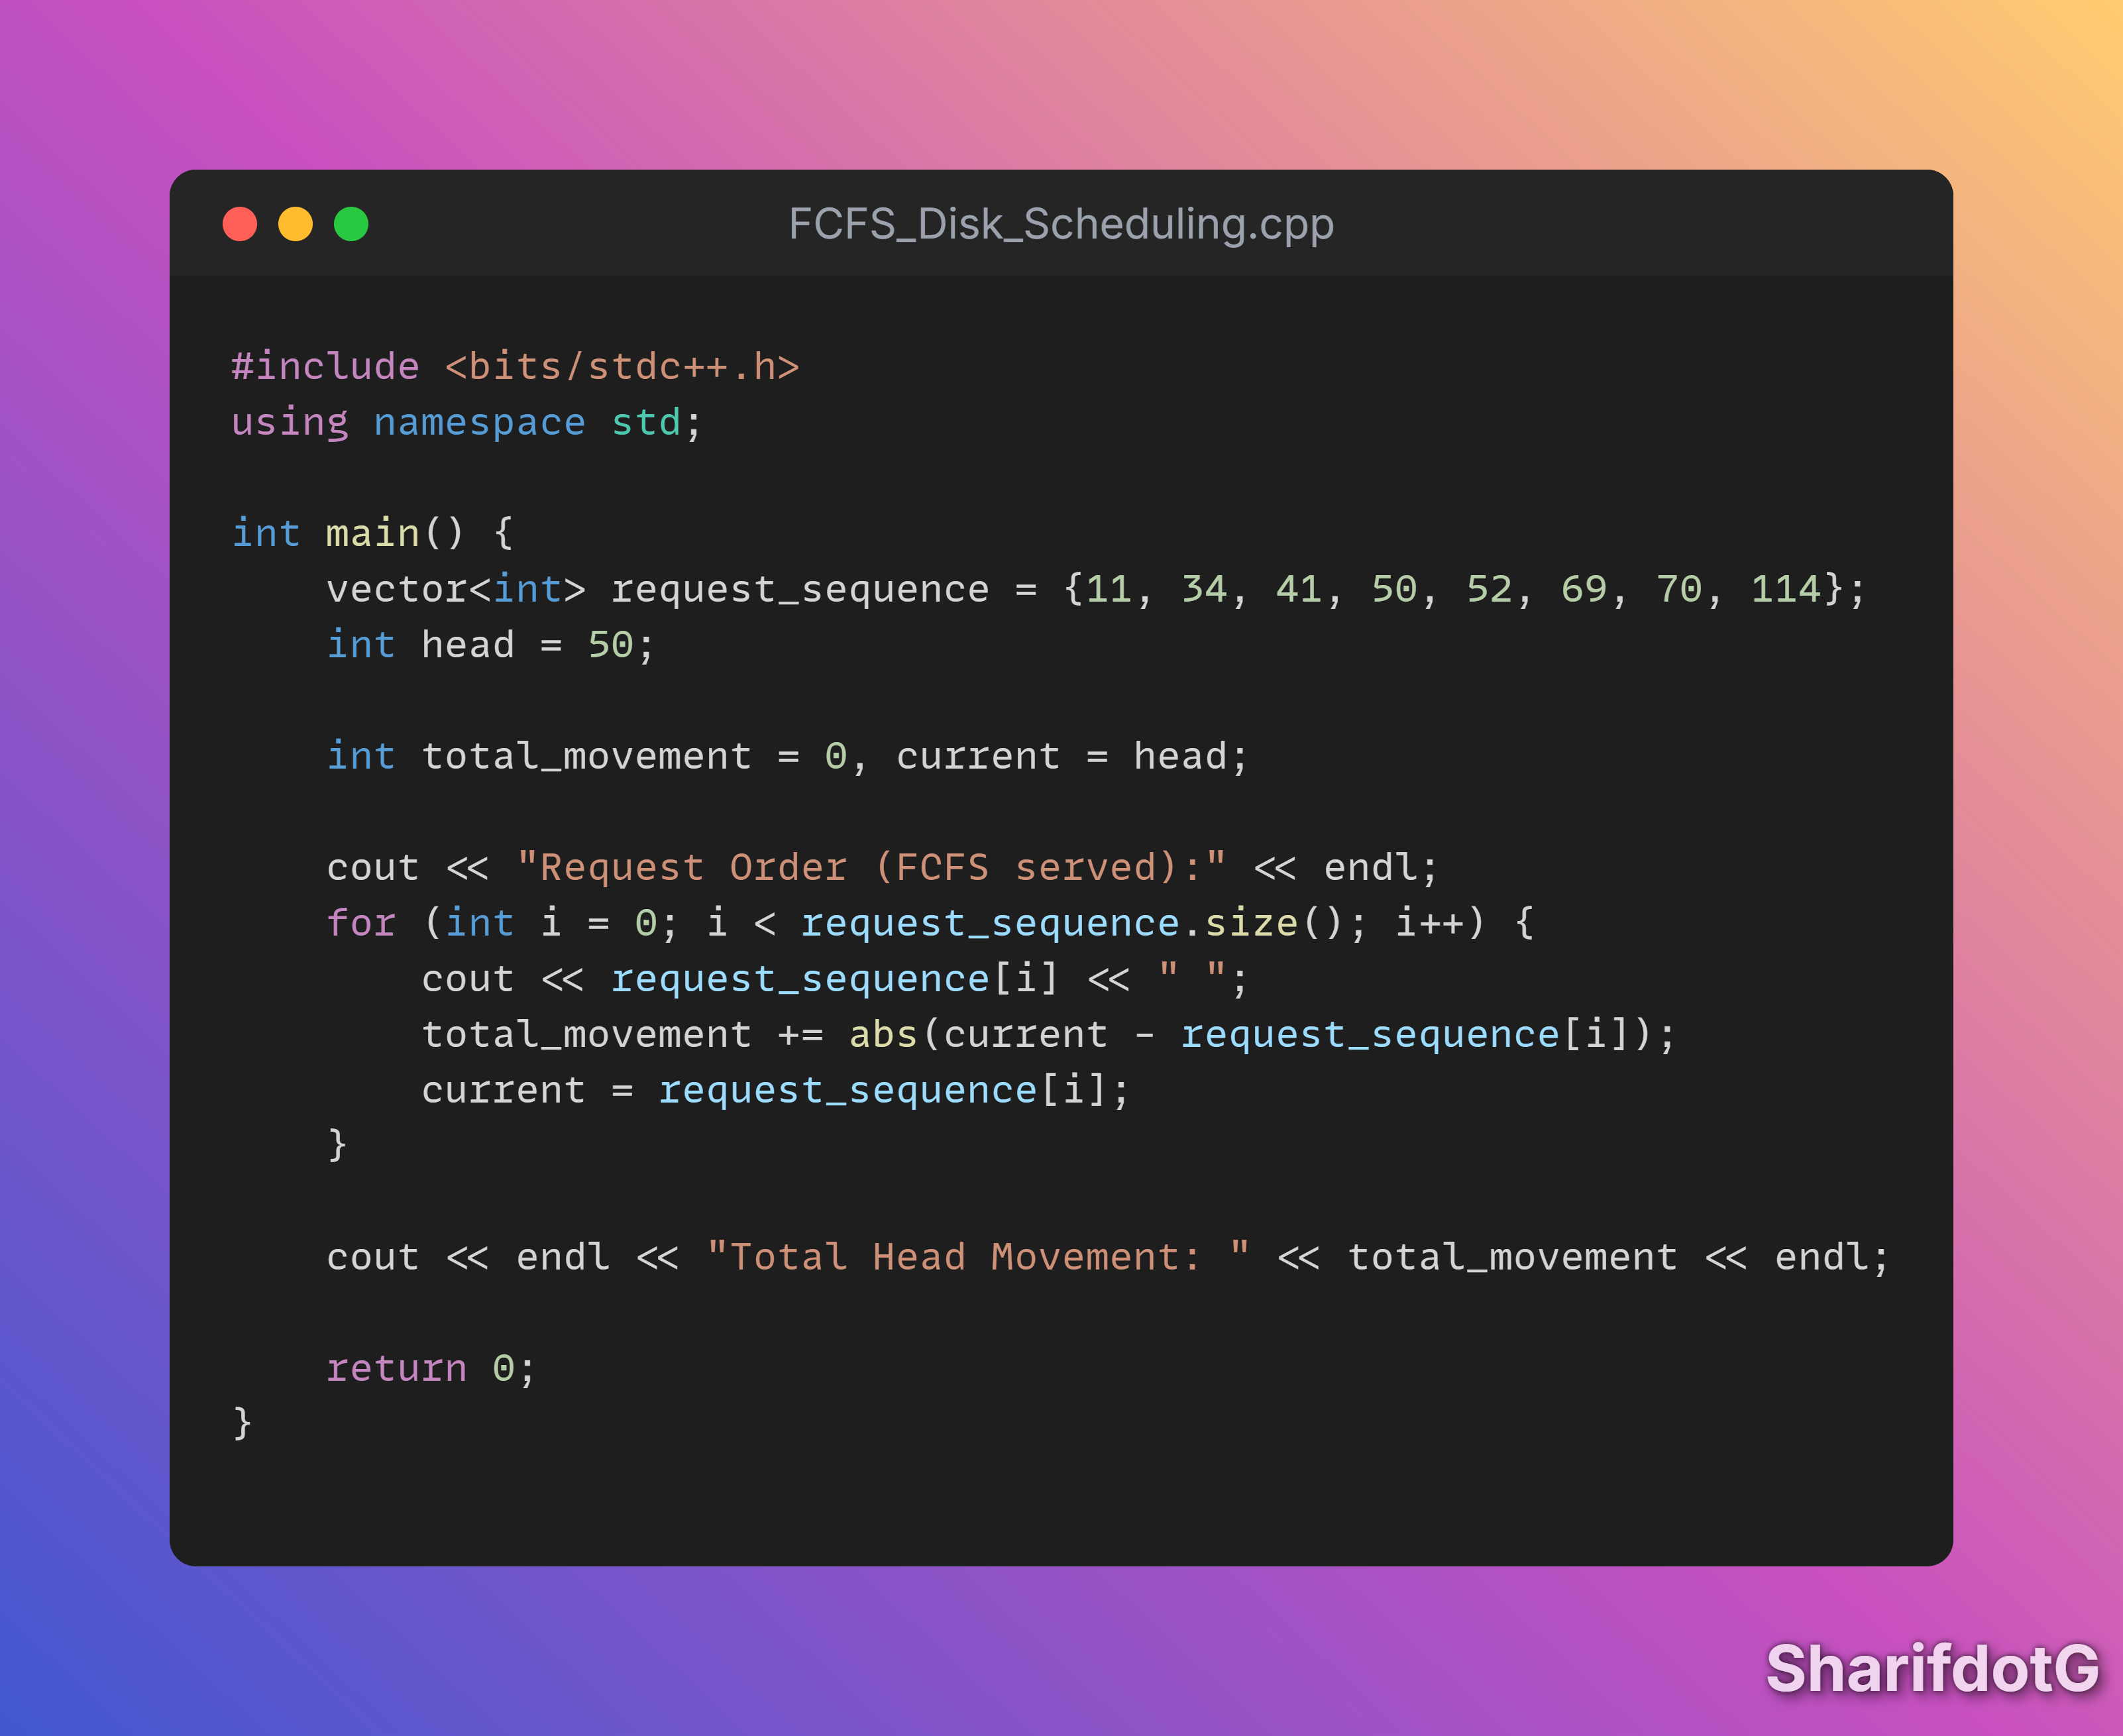
\includegraphics[width=0.85\textwidth]{Code.png}
  \caption{SSTF Disk Scheduling Source Code}
\end{figure}

\section{Output Screenshot}
\begin{figure}[H]
  \centering
  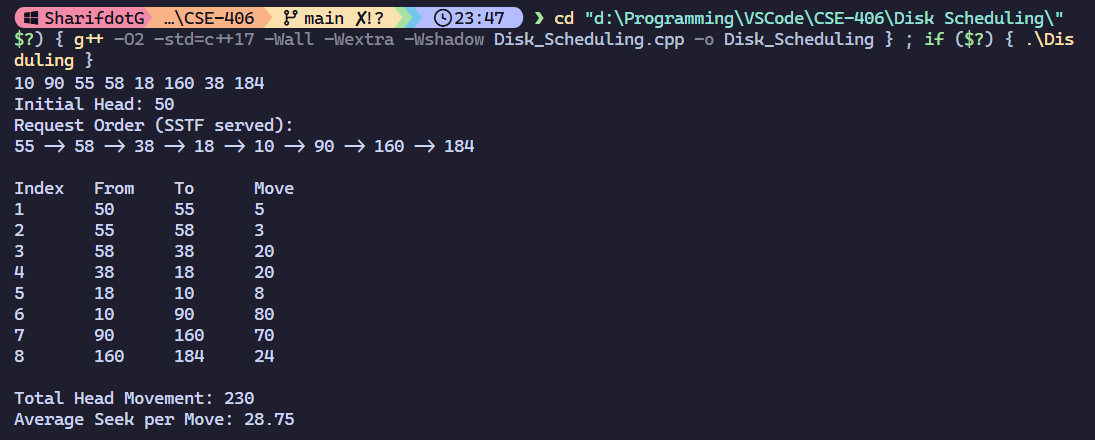
\includegraphics[width=0.85\textwidth]{Screenshot 2025-08-16 234738.png}
  \caption{SSTF Program Output}
\end{figure}

\section{Discussion}
SSTF significantly reduces average seek distance versus naive FCFS when requests are spatially clustered. However:
\begin{itemize}
    \item \textbf{Starvation / Fairness:} Far-out requests may wait if closer requests keep arriving (in dynamic systems).
    \item \textbf{Directional Thrashing:} Head may oscillate locally between nearby cylinders rather than progressing outward, increasing latency for distant requests.
    \item \textbf{Non-Optimality:} Greedy choices can create suboptimal long tail movements.
    \item \textbf{Comparison to SCAN/LOOK:} Elevator algorithms provide more uniform wait times by enforcing directional sweeps, trading a small increase in total movement for fairness.
\end{itemize}
Enhancements could include LOOK/SCAN, C-SCAN variants, or incorporating request arrival times if extended to a dynamic queue. For solid-state drives (SSDs), seek-based heuristics largely lose relevance, shifting optimization toward wear-leveling and parallelism.

\section{Conclusion}
The SSTF disk scheduling implementation demonstrates how a simple greedy heuristic can reduce head travel distance relative to FCFS while introducing fairness concerns. Understanding SSTF provides foundational insight before adopting more balanced algorithms like SCAN or C-SCAN in real disk schedulers.

\end{document}
